\chapter{Resultados y Discusión}
\label{resultadosdiscusion}
\ifpdf
  \graphicspath{{Chapter7/Chapter7Figs/PNG/}{Chapter7/Chapter7Figs/PDF/}{Chapter7/Chapter7Figs/}}
\else
  \graphicspath{{Chapter7/Chapter7Figs/EPS/}{Chapter7/Chapter7Figs/}}
\fi

\markboth{\hfill \thechapter. Resultados y Discusión}{\hfill \thechapter. Resultados y Discusión}

\section{Ambiente de Ejecución}
\label{sec:ambiente_ejecucion}

Las pruebas para la obtención de los resultados se ejecutaron en una computadora personal con la siguiente configuración:
\begin{itemize}
   \item Procesador Intel\textcopyright{}  Core\texttrademark{} i5 2.3 GHz.
    \item Memoria RAM de 8 GB. 
    \item Disco SSD de 256 GB.
    \item Sistema Operativo Linux Mint en su version 18.3 Cinnamon 64-bit.
\end{itemize}

% Para la puesta en marcha de la aplicación \textit{TapeYty} lo requerimientos no funcionales son los siguientes:

% \begin{enumerate}
%     \item 
% \end{enumerate}

% \section{Resultados Obtenidos}
\section{Resultados de Rutas}

% En esta sección se presenta un análisis de los resultados obtenidos con \textit{TapeYty}. 

La Figura \ref{fig:RecorridoActualZona83} muestra el camino trazado por el GPS instalado en el vehículo recolector 129 en la zona 83 de trabajo con una distancia total recorrida de 16.940 km, donde se observa que varios segmentos de calles son atravesados repetidas veces mientras que otros dentro de la zona no son atravesados. En la práctica, los recolectores suelen acumular las bolsas de basura de varias casas en una esquina, evitando que el conductor entrase a ciertas calles, lastimosamente no es posible asegurar que dichos segmentos hayan recibido el servicio. Las avenidas de color naranja que delimitan la zona no forman parte de la recolección pero algunos segmentos de estas avenidas son utilizados para poder acceder a las calles que si deben ser cubiertas por el servicio.

\begin{figure}[htbp]
    \centering
    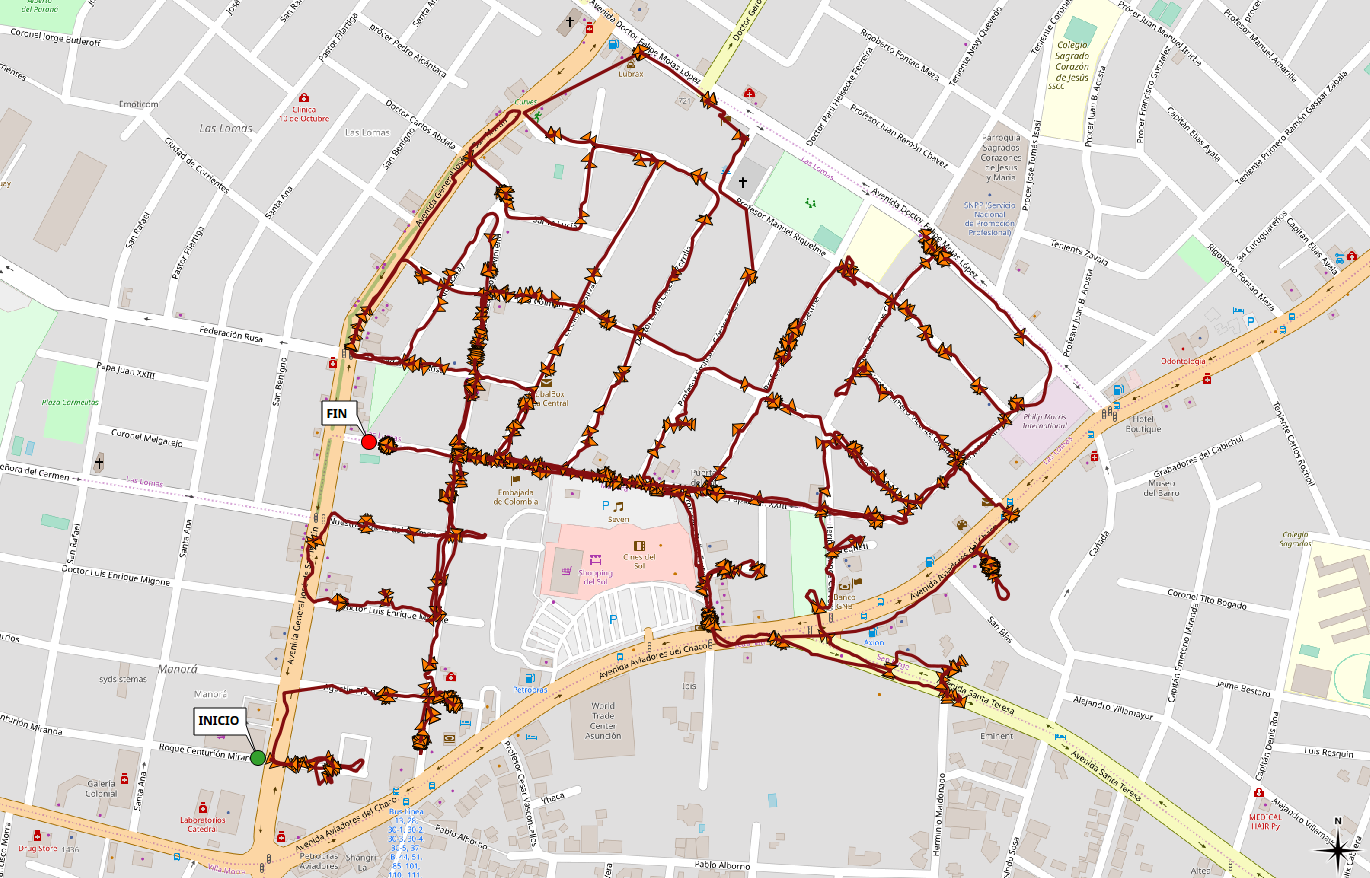
\includegraphics[width=\textwidth]{recorridoActual83.png}
    \caption{Ruta actual. [Fuente: Datos obtenidos en fecha 28/11/2018 del GPS instalado en camión recolector 129 de la DSU]}
    \label{fig:RecorridoActualZona83}
\end{figure}

En la Figura \ref{fig:RecorridoTapeYtyZona83} se muestra el camino generado por \textit{TapeYty} con una cobertura total de las calles que deben ser visitadas en la zona. La secuencia del recorrido se encuentra especificada en los segmentos. La metodología de trabajo se mantiene de acuerdo con lo establecido por la DSU como en la Figura \ref{fig:RecorridoActualZona83}, y por lo tanto, la misma delimitación de zonas.

\begin{figure}[htbp]
    \centering
    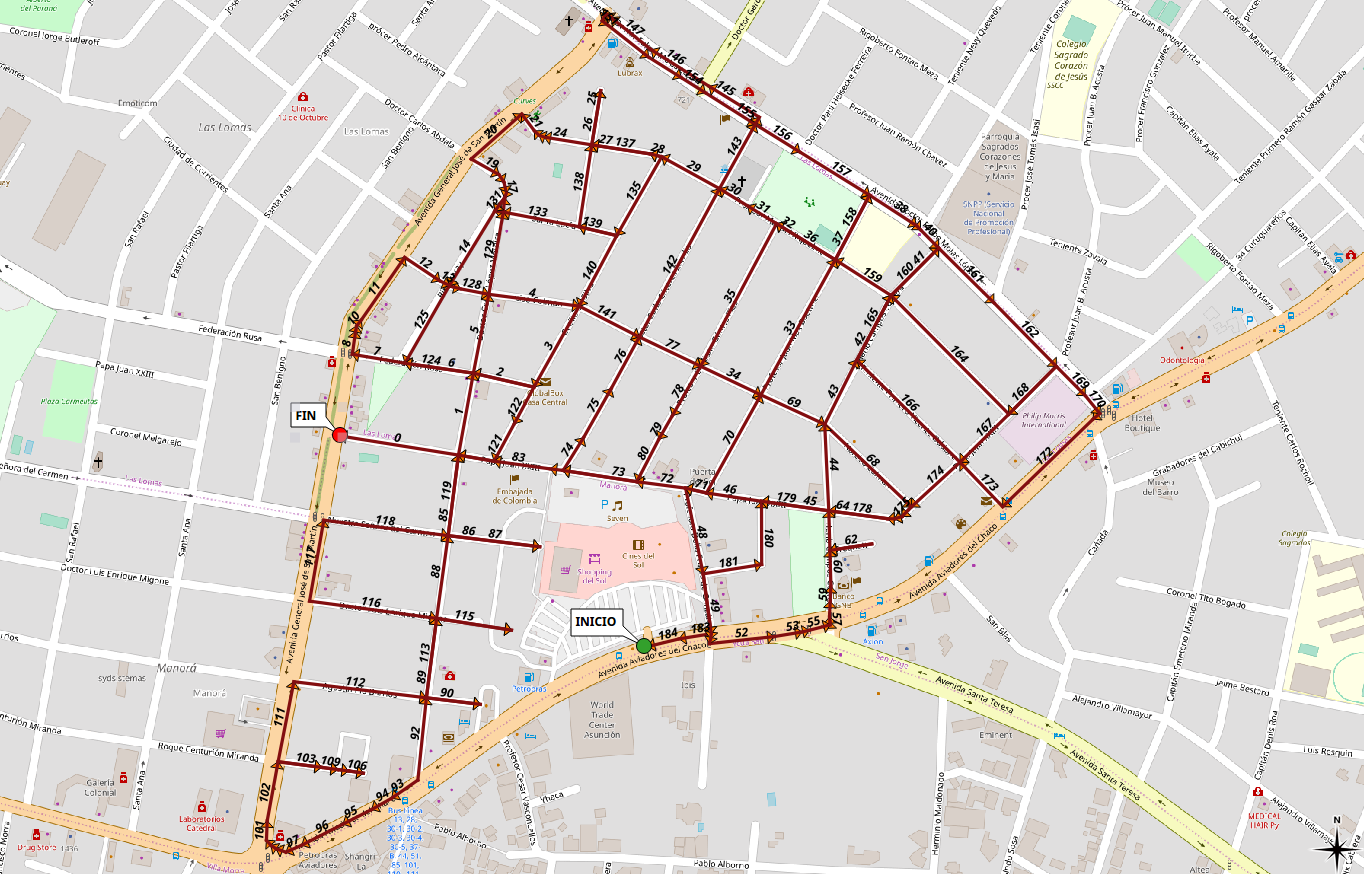
\includegraphics[width=\textwidth]{recorrido83CoberturaTotal.png}
    \caption{Ruta generada por \textit{TapeYty} con cobertura completa.}
    \label{fig:RecorridoTapeYtyZona83}
\end{figure}

Las calles sin salidas, las estrechas y las que limitan una zona pero que no deben ser visitadas necesariamente son gestionadas mediante \textit{TapeYty}. Por ejemplo, en la Figura \ref{fig:RecorridoTapeYtyZona83Opcionales} ciertos segmentos de calles pasan a ser opcionales para el paso de camiones simulando el procedimiento llevado a cabo por el equipo de recolección (ver Figura \ref{fig:RecorridoActualZona83}).

% PAPER
% El punto de inicio de la ruta generada se representa en el mapa con un punto verde, el punto final con un punto rojo y la secuencia a seguir se encuentra especificada en los segmentos de calle. Algunos números de secuencia no son visibles en el mapa debido a que los segmentos son muy pequeños y se requiere de acercamiento para verlos, por ejemplo, el sexto segmento a atravesar no es visible debido a su longitud. El sistema permite exportar un archivo con formato GPX (\textit{GPS eXchange Format}) de la ruta generada que es utilizada para la navegación de la ruta.

Algunas zonas cuentan con varios segmentos de calles de un único sentido y si solo se utilizan los segmentos dentro de la zona, el resultado podría resultar infactible computacionalmente o más costoso en distancia, motivo por el cual se agrega una banda perimetral, tal como en \citet{Braier2017AnArgentina}, de 220 metros representándose a los segmentos de calle dentro de la banda como arcos auxiliares del modelo. Esta situación donde los camiones salen unas cuadras de su zona para volver a entrar es común en la práctica actual de la recolección de residuos.

\begin{figure}[htbp]
    \centering
    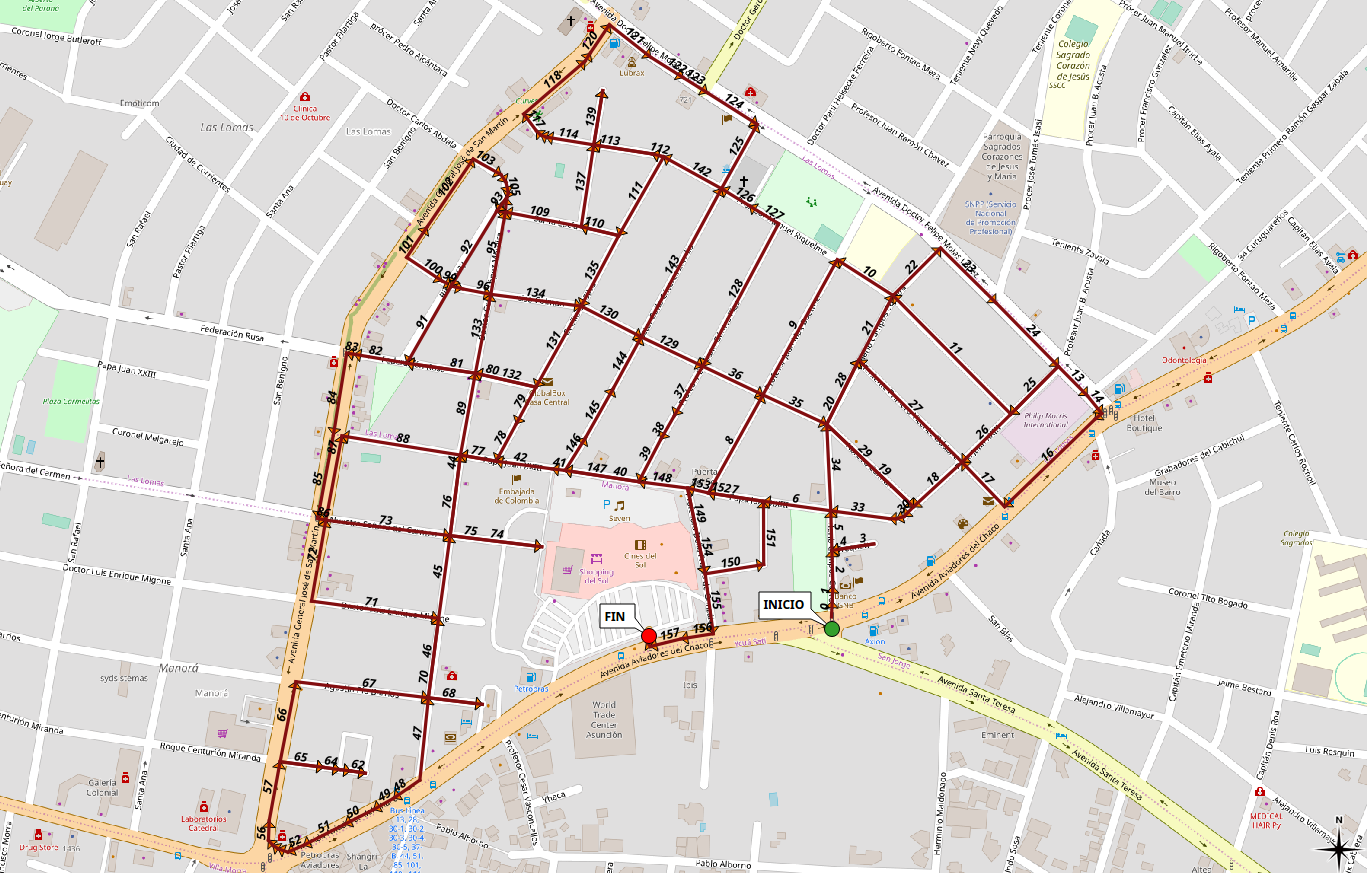
\includegraphics[width=\textwidth]{recorrido83Opcionales.png}
    \caption{Ruta generada por \textit{TapeYty} con segmentos opcionales.}
    \label{fig:RecorridoTapeYtyZona83Opcionales}
\end{figure}

En la Tabla \ref{table:comparacionZona83} se presenta el resultado de la zona 83. En la primera columna se listan las características del modelo: a) número de iteraciones, b) los tiempos de ejecución y c) distancia de la solución. La segunda columna se refiere al escenario en el que todos los segmentos de calles dentro de la zona deben ser visitados por el vehículo recolector y la tercera columna se refiere al escenario en el que 6 segmentos de calles de sentido único y 3 de doble sentido fueron marcados como opcionales desde la aplicación. Si analizamos y comparamos la segunda y tercera columna podemos observar que ambos escenarios coinciden en la cantidad de vértices en el grafo, cantidad de calles de sentido único y de doble sentido, no así en la cantidad de arcos auxiliares debido a la diferencia en la cantidad de segmentos opcionales.

En el primer escenario es posible resolver mediante la técnica de mezcla de subtours recién en la segunda iteración, mientras que en el segundo se puede resolver con la misma técnica ya en la primera iteración. Se observa también que el tiempo de ejecución del modelo es levemente menor para el segundo escenario. Realizar la expansión del grafo a partir de los datos de entrada es el paso que requiere de mayor tiempo en la aplicación. En ambos escenarios se redujo la distancia con respecto al recorrido actual, en el primero en un 20.31\%  y en el segundo un 28.50\%, con 3.44105 km. y 4.82806 km. menos respectivamente.

\begin{table}[htbp]
\caption{Resultados y análisis para la zona 83.}
\begin{tabular}{lll}
\hline
\multirow{2}{*}{Zona 83}                            & \multicolumn{2}{l}{Cobertura de segmentos de calles} \\ \cline{2-3} 
                                                    & Sin opcionales           & Con opcionales           \\ \hline
$|V|$                                                   & 1352                     & 1352                     \\
$|E|$                                                   & 420                      & 420                      \\
$|AM|$                                                  & 256                      & 256                      \\
$|Aaux|$                                                & 1567                     & 1579                     \\
Iteraciones                                         & 2                        & 1                        \\
Tiempo de expansión (s)                      & 20.54530                 & 22.06926                 \\ 
Tiempo de ejecución del modelo (s)            & 0.52790                  & 0.31660                  \\ 
Tiempo de secuenciación (s)                  & 0.04023                  & 0.03425                  \\ 
Distancia (km)                                      & 13.49895                 & 12.11194                 \\ 
Mejora con respecto al actual (\%) & 20.31                    & 28.50                    \\ \hline
\end{tabular}
\label{table:comparacionZona83}
\end{table}

En la Tabla \ref{table:resultadosZonas} se despliegan resultados de tiempos de ejecución de algoritmos y procesos de la optimización de algunas zonas de recolección seleccionadas aleatoriamente. Los resultados de las distintas zonas muestran comportamientos muy similares con respecto a los tiempos. La expansión de zonas siempre requiere de un mayor costo de procesamiento con respecto a los demás tiempos, con registros por encima de 14 segundos y como máximo de 22.5373 segundos. Los tiempos de ejecución del algoritmo de optimización tienen como mayor valor 3.6620 segundos. Por último, los tiempos de secuenciación presentan siempre buen promedio con tiempos entre los rangos 0.0239 y 0.0523 segundos.

% SIMILAR A BRAIER EN ESPANHOL
Si bien la selección para el análisis de resultados fue aleatorio, todas las zonas presentan características similares en tamaño, calles y número de segmentos. Por otra parte, los tiempos de resolución no superaron los 2 minutos para ninguna de las zonas seleccionadas. Estos tiempos son razonables para los requerimientos del sistema. Es importante notar que las rutas obtenidas por este procedimiento fueron bien recibidas por la DSU.

Las rutas actuales informadas en la Tabla \ref{table:comparacionActual} corresponden a datos obtenidos de GPS instalados en los vehículos recolectores por medio de una empresa tercerizada. Estos aparatos están configurados para enviar su ubicación con una frecuencia de 30 segundos generando un margen de error alto con respecto al trazo de las calles de OSM, lo cual influye en la exactitud de las comparaciones. Este problema no se presenció con el recorrido de la zona 83 ya que para ello fue utilizado un GPS configurado por los autores de este trabajo con una frecuencia de 5 segundos.

% DEFINICION DE CAMPUZANO - FPUNA
Para resolver el problema del margen de error se utilizó la estrategia conocida como \textit{Map Matching} (MM). MM es el proceso de identificar la trayectoria seguida por un vehículo en una red de calles a partir de muestras recolectadas acerca de su ubicación. En la Figura \ref{fig:mapMatching} las líneas de color negro representan los datos GPS y las líneas de color verde consiste en la aplicación de la técnica MM con resultados de segmentos coincidentes con el mapa de OSM de la imagen.

La Tabla \ref{table:comparacionActual} presenta la comparación de las distancias de las rutas actuales trazadas con las generadas por \textit{TapeYty}. Como parte del análisis, cabe destacar que los resultados dan un promedio de 19.28\% de mejora con relación al recorrido actual de los camiones considerando los recorridos con calles opcionales. Es interesante destacar que el menor porcentaje de mejora en las rutas con opcionales supera el 10\%.

El ahorro en costos que se puede dar de forma anual es significativo ya que la DSU cuenta con 134 zonas definidas, de las cuales 10 son recorridas 5 días a la semana y el resto 3 veces por semana, durante todo el año. 
%El ahorro en costos que se puede dar de forma anual es significativo.
% El GPS utilizado por los autores de este trabajo en el recorrido de la zona 83 fue configurado con una frecuencia de 5 segundos, motivo por el cual el trazado del camino no cuenta con demasiado margen con respecto al segmento. 

% Los camiones recolectores de la DSU cuentan con dispositivos GPS instalados, reportando la ubicación en tiempo real cada 30 segundos. Para poder identificar la trayectoria seguida es necesario 

\begin{table}[htbp]
\caption{Resultados de ejecución de optimización de zonas.}
\label{table:resultadosZonas}
\resizebox{\textwidth}{!}{%
\begin{tabular}{ccccccccc}
\hline
Nombre de zona     & $|V|$                   & $|E|$                  & $|AM|$                 & $|Aaux|$ & Iteraciones & \begin{tabular}[c]{@{}c@{}}Tiempo de \\ expansión (s)\end{tabular} & \begin{tabular}[c]{@{}c@{}}Tiempo de ejecución \\ del modelo (s)\end{tabular} & \begin{tabular}[c]{@{}c@{}}Tiempo de \\ secuenciación (s)\end{tabular} \\ \hline
71                 & \multirow{2}{*}{1098} & \multirow{2}{*}{404} & \multirow{2}{*}{145} & 1396   & 1           & 18.8936                                                            & 0.2044                                                                        & 0.0330                                                                 \\
71 con opcionales  &                       &                      &                      & 1407   & 1           & 17.9064                                                            & 0.2143                                                                        & 0.0311                                                                 \\ \hline
3                  & \multirow{2}{*}{886}  & \multirow{2}{*}{234} & \multirow{2}{*}{209} & 1105   & 2           & 15.5142                                                            & 0.4226                                                                        & 0.0461                                                                 \\
3 con opcionales   &                       &                      &                      & 1116   & 1           & 14.7611                                                            & 0.2189                                                                        & 0.0417                                                                 \\ \hline
119                & \multirow{2}{*}{1458} & \multirow{2}{*}{654} & \multirow{2}{*}{75}  & 1716   & 3           & 22.5373                                                            & 2.2673                                                                        & 0.0523                                                                 \\
119 con opcionales &                       &                      &                      & 1746   & 1           & 22.5269                                                            & 3.6620                                                                        & 0.0388                                                                 \\ \hline
21                 & \multirow{2}{*}{932}  & \multirow{2}{*}{290} & \multirow{2}{*}{176} & 1067   & 2           & 14.8009                                                            & 0.3358                                                                        & 0.0326                                                                 \\
21 con opcionales  &                       &                      &                      & 1076   & 2           & 14.5501                                                            & 0.3946                                                                        & 0.0239                                                                 \\ \hline
22                 & \multirow{2}{*}{1056} & \multirow{2}{*}{358} & \multirow{2}{*}{170} & 1280   & 3           & 17.1519                                                            & 2.0509                                                                        & 0.0348                                                                 \\
22 con opcionales  &                       &                      &                      & 1308   & 5           & 16.8168                                                            & 1.8977                                                                        & 0.0290                                                                 \\ \hline
83                 & \multirow{2}{*}{1352} & \multirow{2}{*}{420} & \multirow{2}{*}{256} & 1567   & 2           & 20.5453                                                            & 0.5279                                                                        & 0.0402                                                                 \\
83 con opcionales  &                       &                      &                      & 1579   & 1           & 22.0693                                                            & 0.3166                                                                        & 0.0342                                                                 \\ \hline
\end{tabular}%
}
\end{table}

\begin{figure}[htbp]
    \centering
    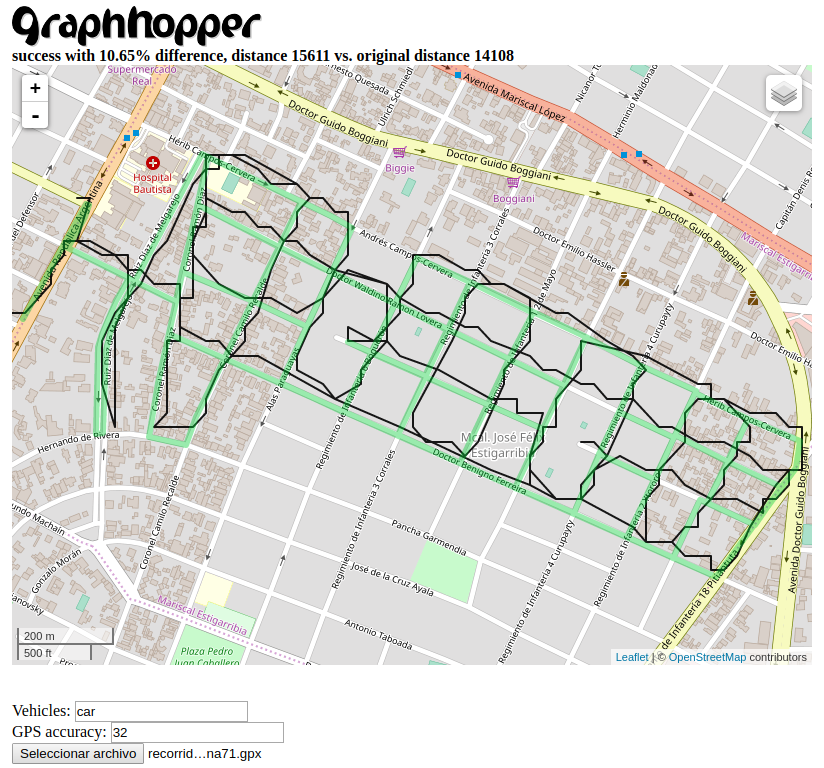
\includegraphics[width=\textwidth]{graphhopper71.png}
    \caption{Técnica \textit{Map Matching} aplicada sobre datos GPS de la DSU utilizando la herramienta \textit{Open Source} Graphhopper.}
    \label{fig:mapMatching}
\end{figure}

\begin{table}[tbp]
\caption{Comparación de resultados obtenidos con el actual.}
\label{table:comparacionActual}
\resizebox{\textwidth}{!}{%
\begin{tabular}{cccc}
\hline
Nombre de zona     & \begin{tabular}[c]{@{}c@{}}Distancia actual (km) \\ con Map matching\end{tabular} & Distancia generada (km) & \begin{tabular}[c]{@{}c@{}}Mejora con respecto \\ al actual (\%)\end{tabular} \\ \hline
71                 & \multirow{2}{*}{15.611}                                                           & 14.358                  & 8.02                                                                          \\
71 con opcionales  &                                                                                   & 13.320                  & 14.67                                                                         \\ \hline
3                  & \multirow{2}{*}{19.486}                                                           & 17.851                  & 8.39                                                                          \\
3 con opcionales   &                                                                                   & 16.879                  & 13.38                                                                         \\ \hline
119                & \multirow{2}{*}{16.940}                                                           & 14.704                  & 13.19                                                                         \\
119 con opcionales &                                                                                   & 13.825                  & 18.38                                                                         \\ \hline
21                 & \multirow{2}{*}{14.895}                                                           & 13.003                  & 12.7                                                                          \\
21 con opcionales  &                                                                                   & 11.675                  & 21.62                                                                         \\ \hline
22                 & \multirow{2}{*}{14.382}                                                           & 12.622                  & 12.24                                                                         \\
22 con opcionales  &                                                                                   & 11.635                  & 19.1                                                                          \\ \hline
83                 & \multirow{2}{*}{16.940}                                                           & 13.499                  & 20.31                                                                         \\
83 con opcionales  &                                                                                   & 12.112                  & 28.5                                                                          \\ \hline
\end{tabular}%
}
\end{table}

\section{Calidad de Software}

Existen varias definiciones para el concepto de Calidad de Software y la mayoría suele coincidir en la idea de adecuación a los requerimientos. La calidad de software está definida en \citet{Pressman2010IngenieriaPractico} como ``el proceso eficaz de software que se aplica de manera que crea un producto útil que proporciona valor medible a quienes lo producen y a quienes lo utilizan''. La ISO/IEC 9126 la define como ``el grado con el que un sistema, componente o proceso cumple los requerimientos especificados y las necesidades o expectativas del cliente o usuario''. 

Entre los atributos de la Calidad del Software tenemos: seguridad, fiabilidad, flexibilidad, robustez, comprensibilidad, testeabilidad, adaptabilidad, modularidad, complejidad, portababilidad, usabilidad, reusabilidad, eficiencia y facilidad.

\subsection{Calidad de código fuente}

A continuación se muestra un reporte con las métricas de algunos atributos de calidad en los proyectos \textit{backend} y \textit{frontend} de la aplicación. Las incidencias encontradas en ambos proyectos se fueron solucionando y corrigiendo. Se utilizaron las reglas por defecto proporcionadas por la herramienta utilizada SonarQube. (Ver Figuras \ref{fig:QAbackend}, \ref{fig:QAfrontend})

SonarQube define tres tipos de problemas:

\begin{itemize}
    \item \textit{Bug}: Un error de codificación que romperá su código y debe solucionarse de inmediato.
    \item \textit{Vulnerability}: Un punto en su código que está abierto al ataque.
    \item \textit{Code smell}: Un problema de mantenibilidad que hace que su código sea confuso y difícil de mantener.
\end{itemize}

Cada problema corresponde a una de las cinco severidades:

\begin{itemize}
    \item \textit{Blocker}: Error con una alta probabilidad de afectar el comportamiento de la aplicación en producción: pérdida de memoria, conexión JDBC no cerrada, etc. El código debe ser arreglado de inmediato.
    \item \textit{Critical}: Ya sea un error con poca probabilidad de afectar el comportamiento de la aplicación en producción o un problema que representa un defecto de seguridad: bloque de captura vacío, inyección de SQL, etc. El código debe revisarse de inmediato.
    \item \textit{Major}: Defecto de calidad que puede tener un gran impacto en la productividad del desarrollador: pieza de código descubierta, bloques duplicados, parámetros no utilizados.
    \item \textit{Minor}: Defecto de calidad que puede afectar ligeramente la productividad del desarrollador: las líneas no deben ser demasiado largas, las declaraciones de ``cambio'' deben tener al menos 3 casos, entre otros.
    \item \textit{Info}: Ni un error ni un defecto de calidad, solo un hallazgo.
\end{itemize}

\begin{figure}[H]
    \centering
    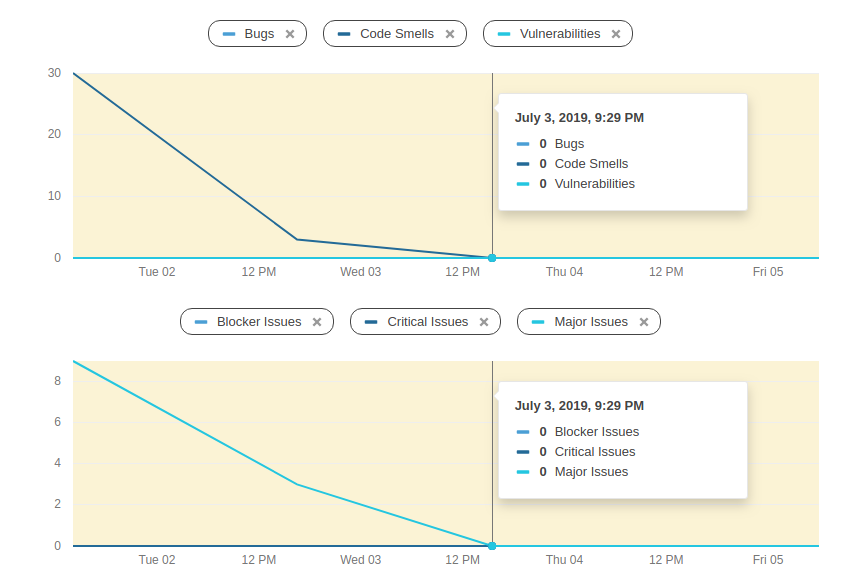
\includegraphics[width=\textwidth]{reporteQA_BE.png}
    \caption{Reporte de inspección de código con SonarQube del \textit{Backend}.}
    \label{fig:QAbackend}
\end{figure}

\begin{figure}[H]
    \centering
    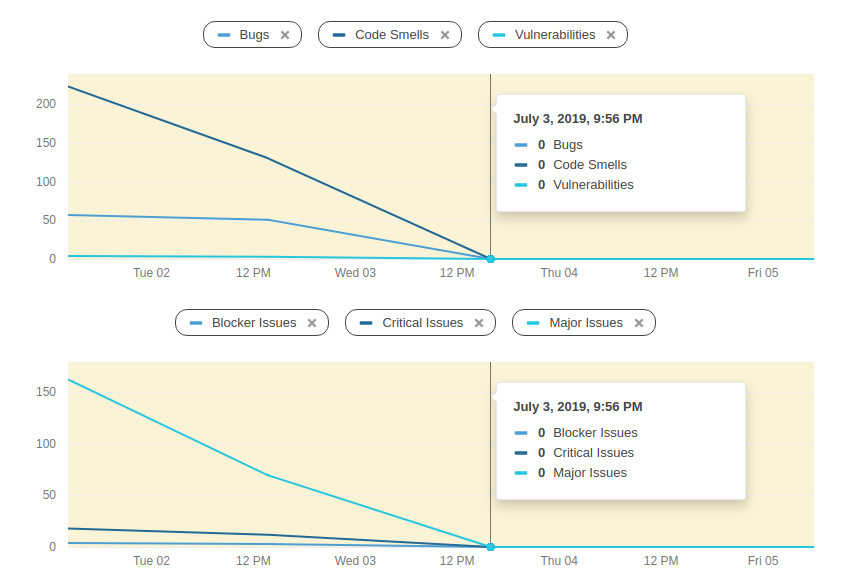
\includegraphics[width=\textwidth]{reporteQA_FE2.png}
    \caption{Reporte de inspección de código con SonarQube del \textit{Frontend}.}
    \label{fig:QAfrontend}
\end{figure}

\subsection{Pruebas de rendimiento}

Las pruebas de rendimiento generalmente se realizan para ayudar a identificar cuellos de botella en un sistema, establecer una línea de base para pruebas futuras, respaldar un esfuerzo de ajuste del rendimiento, determinar el cumplimiento de los objetivos y requisitos de rendimiento y/o recopilar otros datos relacionados con el rendimiento para ayudar a las partes interesadas a tomar decisiones informadas relacionadas a la calidad general de la aplicación que se está probando \citep{Corporation2007PerformanceApplications}.

% Las pruebas de rendimiento consisten en simular carga en el sistema bajo pruebas para analizar el desempeño del mismo durante la ejecución de la prueba, pudiendo encontrar cuellos de botella y oportunidades de mejora. La forma en la que estaremos aportando calidad es principalmente buscando fallos. La idea es encontrar la mayor cantidad de fallos que más calidad le aporten al producto \citep{ToledoRodriguez2014IntroduccionInformacion}.

Se preparó un plan de pruebas de rendimiento siguiendo las actividades presentadas en \citet{Corporation2007PerformanceApplications}:

\begin{enumerate}
    \item \textbf{Identificar el entorno de prueba:}
        Como servidor de aplicación se utiliza el ambiente de ejecución mencionado más arriba en la sección \ref{sec:ambiente_ejecucion}. En la misma red del servidor se cuenta con otra estación de trabajo, donde se instala la herramienta Jmeter \citep{ApacheJMeter} para analizar y medir el desempeño de la aplicación.
    \item \textbf{Identificar los criterios de aceptación del rendimiento:}
        La DSU cuenta con dos administradores del sistema encargados de la gestión de rutas de recolección. Además, teniendo en cuenta la cantidad de zonas y turnos de trabajos un máximo de 23 conductores se conectarán en simultáneo para descargar su ruta asignada. El usuario espera obtener una nueva ruta en menos de 120 segundos.
    \item \textbf{Planificación y diseño de pruebas:}
        En esta actividad se decide emplear dos tipos de pruebas de rendimiento: de carga y de estrés. Las pruebas de carga consisten en simular la realidad a la que estará expuesto el sistema cuando esté en producción y las pruebas de estrés son pruebas para encontrar el volumen de datos o de tiempo en que la aplicación comienza a fallar o es incapaz de responder a las peticiones \citep{ToledoRodriguez2014IntroduccionInformacion}. Se plantean dos escenarios: A) Uno en el que los usuarios visualizan una ruta ya generada previamente; y B) en el que los usuarios generan una nueva ruta.
    \item \textbf{Configurar el entorno de prueba:}
        Se prepara el entorno de prueba, las herramientas y los recursos necesarios para ejecutar cada estrategia. Se realizan ajustes en los servidores web y de aplicación en el servidor para aprovechar las características de su procesador y mejorar así el rendimiento. Se instala en Jmeter el plugin SSHMon \citep{Jmeter-sshmon} para obtener resultados de monitoreo de CPU y uso de disco del servidor.
    \item \textbf{Implementar el diseño de prueba:}
        Se implementa la planificación y diseño de las pruebas.
    % \item Ejecute la prueba:
    % \item Analizar resultados, informar y volver a probar:
\end{enumerate}

A continuación, se detallan los resultados de la ejecución de las pruebas y un análisis de los mismos, que corresponden a las últimas actividades del plan de pruebas de rendimiento \citep{Corporation2007PerformanceApplications}.

Para el escenario A los usuarios realizan peticiones a los siguientes servicios del sistema:
\begin{itemize}
    \item Seleccionar una zona.
    \item Listar históricos de rutas para una zona seleccionada.
    \item Ver un camino.
    \item Exportar una ruta a GPX.
\end{itemize}
% \label{prueba:escA} 

Para el escenario B los usuarios realizan peticiones al servicio de:
\begin{itemize}
    \item Generar nueva ruta.
\end{itemize}
% \label{prueba:escB} 

\subsubsection{Resultados de pruebas de carga}
\label{ref:resultadosPruebaCarga}

Los resultados de rendimiento de carga del escenario A se visualizan en la Figura \ref{fig:25UsuariosCargaA}, donde se observa que la cantidad de peticiones por unidad de tiempo (\textit{Throughput}) para cada etiqueta (\textit{label}) es aceptable. La desviación estándar (\textit{Std. Dev}) presenta valores pequeños con respecto al promedio (\textit{Average}) de cada etiqueta, concluyendo en que los tiempos de respuesta no son dispersos. En la Figura \ref{fig:25UsuariosCPUA} se observa el porcentaje de utilización de CPU y el número total de transferencias por segundo del disco (I/O) durante el tiempo de ejecución de las pruebas. Al iniciar el lanzamiento de las peticiones concurrentes la CPU es utilizada en un 63 \%, pero en unos pocos segundos va liberando recursos utilizando menos del 20\%.

% Esto muestra el conjunto de casos excepcionales que se estaban desviando del valor promedio del tiempo de respuesta de la muestra. Cuanto menor es este valor, más coherentes son los datos. La desviación estándar debe ser menor o igual a la mitad del tiempo promedio para una etiqueta.

\begin{figure}[H]
    \centering
    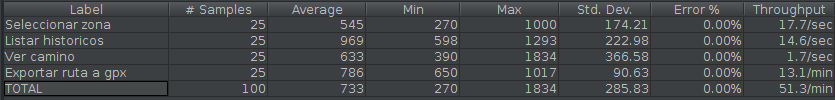
\includegraphics[width=\textwidth]{25_usuarios_editado_.png}
    \caption{Reporte de rendimiento de carga con 25 usuarios concurrentes ejecutando el escenario A.}
    \label{fig:25UsuariosCargaA}
\end{figure}

\begin{figure}[H]
    \centering
    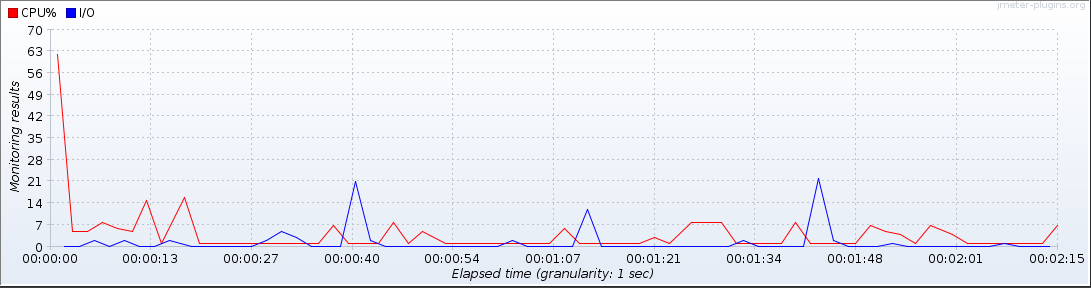
\includegraphics[width=\textwidth]{25_usuarios_plan_a_cpu.png}
    \caption{Reporte de utilización de recursos en el servidor con una carga de 25 usuarios concurrentes ejecutando el escenario A.}
    \label{fig:25UsuariosCPUA}
\end{figure}

Para el escenario B se pueden observar los resultados en las Figuras \ref{fig:5UsuariosCargaB} y \ref{fig:5UsuariosCPUB}. Se observa que la desviación estándar es aceptable y que la cantidad de peticiones por minuto que puede manejar el servidor es mucho menor a las peticiones del escenario A. En la Figura \ref{fig:5UsuariosCargaB}, como era de esperarse, se muestra que generar nuevas rutas es el proceso más costoso del sistema requiriendo más recursos de CPU en el servidor.

\begin{figure}[H]
    \centering
    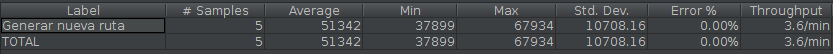
\includegraphics[width=\textwidth]{Chapter7/Chapter7Figs/5_usuarios_doc_editado_.png}
    \caption{Reporte de rendimiento de carga con 5 usuarios concurrentes ejecutando el escenario B.}
    \label{fig:5UsuariosCargaB}
\end{figure}

\begin{figure}[H]
    \centering
    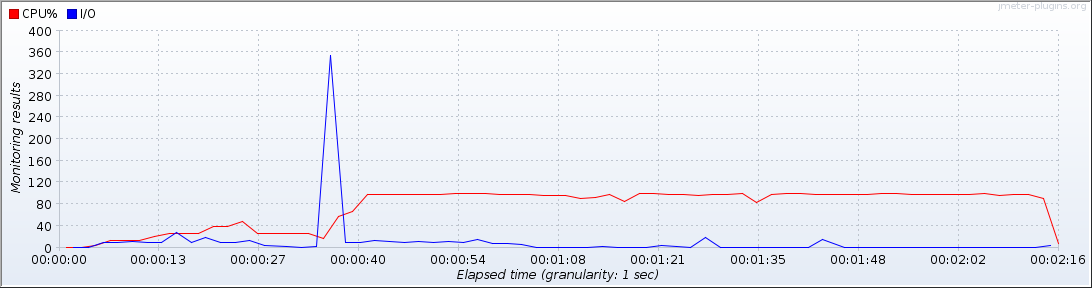
\includegraphics[width=\textwidth]{5_usuarios_plan_b_cpu_.png}
    \caption{Reporte de utilización de recursos en el servidor con una carga de 5 usuarios concurrentes ejecutando el escenario B.}
    \label{fig:5UsuariosCPUB}
\end{figure}

\subsubsection{Resultados de pruebas de estrés}
\label{ref:resultadosPruebaEstres}

El escenario de prueba A se ejecutó sin errores con 100 y 500 usuarios concurrentemente como se puede ver en las Figuras \ref{fig:100UsuariosEstresA} y \ref{fig:500UsuariosEstresA} respectivamente. Recién cuando se ejecutó con 510 usuarios se observa que hubo un promedio total de 0.39 \% de error (ver Figura \ref{fig:510UsuariosEstresA}). El motivo de fallo es que el servidor se configuró hasta un límite de 500 sesiones concurrentes.

\begin{figure}[H]
    \centering
    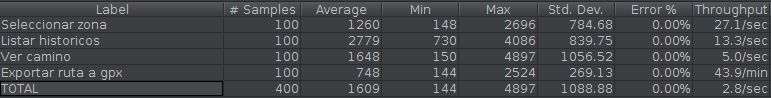
\includegraphics[width=\textwidth]{100_usuarios_sin_optimizacion_editado_.png}
    \caption{Reporte de pruebas de estrés con 100 usuarios concurrentes ejecutando el escenario A.}
    \label{fig:100UsuariosEstresA}
\end{figure}

\begin{figure}[H]
    \centering
    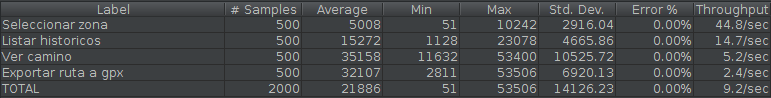
\includegraphics[width=\textwidth]{500_usuarios_sin_optimizacion_editado_.png}
    \caption{Reporte de pruebas de estrés con 500 usuarios concurrentes ejecutando el escenario A.}
    \label{fig:500UsuariosEstresA}
\end{figure}

\begin{figure}[H]
    \centering
    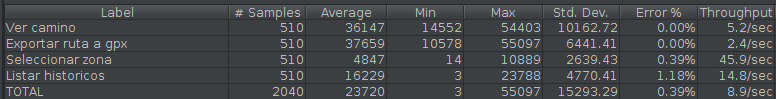
\includegraphics[width=\textwidth]{510_usuarios_sin_optimizacion_editado_.png}
    \caption{Reporte de pruebas de estrés con 510 usuarios concurrentes ejecutando el escenario A}
    \label{fig:510UsuariosEstresA}
\end{figure}

El escenario de prueba B se ejecutó sin errores con 25 usuarios concurrentemente como se puede ver en la Figura \ref{fig:25UsuariosEstresB}. Cuando se ejecutó con 40 usuarios se observa un 35\% de errores, todos ellos debido a \textit{Timeout} a consecuencia de que el servidor se configuró con un tiempo máximo de respuesta de 300 segundos (5 minutos).

\begin{figure}[H]
    \centering
    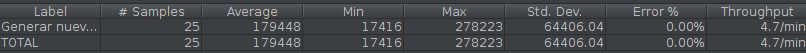
\includegraphics[width=\textwidth]{25_usuarios_generar_ruta.png}
    \caption{Reporte de pruebas de estrés con 25 usuarios concurrentes ejecutando el escenario B.}
    \label{fig:25UsuariosEstresB}
\end{figure}

\begin{figure}[H]
    \centering
    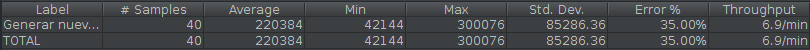
\includegraphics[width=\textwidth]{40_usuarios_plan_b_.png}
    \caption{Reporte de pruebas de estrés con 40 usuarios concurrentes ejecutando el escenario B.}
    \label{fig:40UsuariosEstresB}
\end{figure}

Con la finalización de las pruebas se concluye que un servidor con las características y configuraciones aplicadas en el ambiente de prueba es más que suficiente para cumplir con los requerimientos relevados en la DSU indicados en el plan de pruebas. Es importante destacar que generar rutas es un proceso que requiere de un alto consumo de recursos computacionales, es por ello que se recomienda que el motor de optimización esté implantado en un servidor dedicado. Otra alternativa a considerar en caso de que el número de usuarios concurrentes aumente considerablemente es utilizar una heurística para resolver el problema de ruta.

\subsection{Usabilidad}

% El objetivo de la evaluación de usabilidad de este trabajo es conocer la percepción subjetiva de los usuarios acerca de la usabilidad general del sistema \textit{TapeYty}.
% Para ello se utilizó la métrica de “Actitud o satisfacción del usuario”

% The ISO 9241-11 standard defines usability as “the extent to which a product can be used by specified users to achieve specified goals with effectiveness, efficiency and satisfaction in a specified context of use”
%  dice que la usabilidad se refiere al alcance en el que un producto puede ser utilizado por usuarios específicos para alcanzar metas específicas con efectividad, eficiencia y satisfacción en un contexto específico de uso. 

El estándar ISO 9241-11 define la usabilidad como ``la medida en que un producto puede ser utilizado por usuarios específicos para lograr objetivos específicos con efectividad, eficiencia y satisfacción en un contexto de uso específico''

La norma ISO/IEC 9126-4 recomienda que las métricas de usabilidad incluyan:

\begin{itemize}
    \item Efectividad: la precisión e integridad con la que los usuarios logran objetivos específicos.
    \item Eficiencia: los recursos gastados en relación con la precisión y la integridad con la que los usuarios alcanzan los objetivos.
    \item Satisfacción: la comodidad y la aceptabilidad del uso.
\end{itemize}

% Si la medición de la satisfacción del usuario es importante pero no hay un gran presupuesto asignado, entonces se debe usar SUS.
Dado que la satisfacción del usuarios es importante para la validación de este trabajo y no se cuenta con un gran presupuesto para ello, se realiza la medición del mismo utilizando la Escala de Usabilidad del Sistema (SUS, \textit{System Usability Scale}) elaborada por \cite{Brooke1986SUSScale} para obtener una visión global de evaluaciones subjetivas de usabilidad de la interfaz de \textit{TapeYty}.

SUS consiste en solo diez preguntas, un sistema de puntuación de 5 puntos (desde ``Completamente de acuerdo'' hasta ``Completamente en desacuerdo''), y un algoritmo rápido de puntuación. SUS es una escala muy fácil, es simple de administrar a los participantes, por lo que es ideal para usar con tamaños de muestra pequeños. En la literatura se ha encontrado que dan resultados muy precisos y de mucho valor.
% Los elementos impares redactados positivamente y elementos pares redactados negativamente.

La formulación matemática para obtener el puntaje general de SUS puede ser descrito como sigue:

\begin{equation} \label{eqSus1}
\begin{gathered}
y_{i} = x_{i} - 1 \\
\forall i = {1, 3, 5, 7,9}
\end{gathered}
\end{equation} 
\hbox{}

\begin{equation} \label{eqSus2}
\begin{gathered}
y_{i} = 5 - x_{i} \\
\forall i = {2, 4, 6, 8, 10}
\end{gathered}
\end{equation} 
\hbox{}

\begin{equation} \label{eqSus3}
\begin{gathered}
SUS =  \sum_{i=1}^{10} y_{i} \times 2.5 \\
\end{gathered}
\end{equation} 

En (\ref{eqSus1}), (\ref{eqSus2}) y (\ref{eqSus3}) se utiliza la siguiente notación: 
\begin{itemize}
    \item $i$ representa el número de la pregunta.
    \item $x$ el valor de la respuesta.
    \item $y$ el puntaje asignado a la respuesta.
    \item $SUS$ puntaje general de SUS.
\end{itemize}

% En el Apendice XX se encuentra el formulario completado por los evaluadores, que fueron las personas que estarán a cargo de la administración de TapeYty.

La subescala de usabilidad se corresponden con los ítem 1, 2, 3, 5, 6, 7, 8, 9 (ecuación \ref{eqSeU}); y la subescala de facilidad de aprendizaje se corresponden con los ítem 4 y 10 (ecuación \ref{eqSeFA}) \citep{Lewis2009TheScale}.

\begin{equation} \label{eqSeU}
\begin{gathered}
SeU = (y_{1} + y_{2} + y_{3} + y_{5} + y_{6} + y_{7} + y_{8} + y_{9}) \times 3.125 \\
\end{gathered}
\end{equation} 
\hbox{}

\begin{equation} \label{eqSeFA}
\begin{gathered}
SeFA = (y_{4} + y_{10}) \times 12.5 \\
\end{gathered}
\end{equation} 
\hbox{}

En la tabla \ref{tabla:SUSResultado} se presentan los resultados de la evaluación utilizando las ecuaciones \ref{eqSus3}, \ref{eqSeU} y \ref{eqSeFA} respectivamente.

\begin{table}[]
\caption{Resultados SUS}
\label{tabla:SUSResultado}
\centering
\begin{tabular}{|c|c|c|}
\hline
SUS General & Sub Escala Usabilidad & Facilidad de aprendizaje \\ \hline
85.83             & 90.63                & 66.67                       \\ \hline
\end{tabular}
\end{table}

El puntaje general de SUS fue de 85.83. Teniendo en cuenta el análisis de \cite{Bangor2009DeterminingScale} (ver Figura \ref{fig:susScore}), el rango entre 80 a 89 corresponde a una B, es decir, el sistema es ``Aceptable'', utilizando los adjetivos de calificación de este análisis el sistema es lo ``Mejor Posible''.

Luego el puntaje general de SUS es descompuesto en sus componentes de usabilidad y capacidad de aprendizaje:
\begin{itemize}
    \item El resultado de ``Sub-escala de usabilidad'' fue de 90.63, teniendo en cuenta el análisis de \cite{Bangor2009DeterminingScale}, el rango entre 90 a 100 corresponde a una A, es decir, el sistema es ``Aceptable'', utilizando los adjetivos de calificación de este análisis el sistema es lo ``Mejor Posible''.
    \item El resultado de ``Facilidad de aprendizaje'' fue de 66.67, teniendo en cuenta el análisis de \cite{Bangor2009DeterminingScale}, el rango de 52 hasta 73, el sistema está considerada como ``Buena'', era de esperarse ya que se requiere de conocimientos previos de herramientas GIS para la utilización del sistema, en \citep{Borsci2009OnModels} mostraron que los dos factores (usabilidad y facillidad de aprendizaje) son independientes. 
\end{itemize}{}


\begin{figure}[]
    \centering
    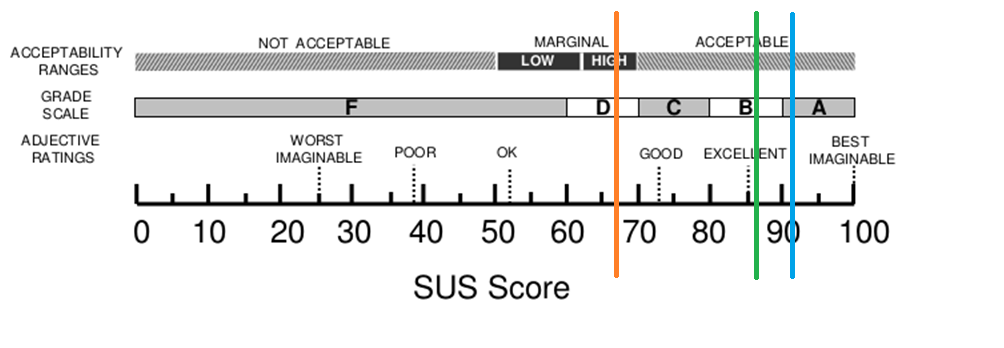
\includegraphics[width=\textwidth]{SUS_resultados.png}
    \caption{Una comparación de las calificaciones de los adjetivos, los puntajes de aceptabilidad y las escalas de calificación escolar, en relación con el puntaje promedio del SUS [Fuente:\citep{Bangor2009DeterminingScale}]}
    \label{fig:susScore}
\end{figure}
